\documentclass[a4paper]{article}

\usepackage[utf8]{inputenc}
\usepackage[portuges]{babel}
\usepackage{a4wide}
\usepackage{fancyvrb}
\usepackage{graphicx}



\title{Projeto de Laboratórios de Informática 1\\Grupo 48}
\author{José Pedro Moreira Resende a77486 \and Manuel Gouveia Carneiro de Sousa a78869}

\begin{document}

\maketitle

\begin{abstract}
Este trabalho tem o principal objetivo o desenvolvimento do jogo \textit{Sokoban} na linguagem funcional \textit{Haskell}. Neste jogo, pretendemos colocar várias caixas em diferentes posições, caixas estas que são arrastadas por um boneco. 

Este relatório pretende sumarizar todos os parâmetros estudados e desenvolvidos durante este projeto, bem como os passos que foram seguidos e tomados. Através de várias tarefas propostas pelos docentes, fomos desenvolvendo o código necessário para: Validação do mapa bem como as coordenadas das posições do boneco e diferentes caixas; Validação de possíveis comandos a dar ao boneco para que este se movesse, bem como as caixas; E, por fim, a criação do ambiente gráfico (GUI) para o jogo.

\end{abstract}

\tableofcontents
\newpage

\section{Introdução}
\label{sec:intro}

Neste projeto, com o objetivo da criação de um jogo e todas as suas componentes, os problemas foram repartidos em diferentes tarefas (como anteriormente referido), tarefas estas que propunham uma forma eficiente da resolução do nosso problema. Todo o código desenvolvido nas diferentes tarefas era submetido e avaliado na plataforma \textit{Mooshak}, onde por sua vez era cotado conforme os testes em que era válido, ou não. Pretendia-se, portanto, resolver diferentes problemas, os quais eram a resolução de todo o nosso projeto.

A abordagem feita por nós neste projeto foi seguida pelos enunciados propostos no \textit{Mooshak}, em que nos era fornecido uma possível estrutura para o começo do desenvolvimento do nosso código. Após uma estruturação do nosso raciocínio e das diferentes ideias, começamos a desenvolver o código das diferentes tarefas, tendo em conta um procedimento lógico que abordasse todos os casos necessários para o bom funcionamento da tarefa, e do problema.

Neste relatório, vamos descrever o problema em causa, bem como objetivos que pretendemos alcançar. Vamos falar da concepção e desenvolvimento do código e do problema, explicando cada tarefa realizada, a forma e estrutura de como as nossas tarefas foram feitas, e os diferentes testes que fomos realizando ao longo de todo o desenvolvimento. 


\section{Descrição do Problema}
\label{sec:problema}

No projeto em causa, tinhamos como problema principal, o desenvolvimento e funcionamento de um jogo. Para isto, o problema foi abordado conforme os enunciados dispostos na plataforma Mooshak. O jogo, que consiste num tabuleiro com caixas, um boneco, e diferentes espaços vazios para onde as caixas têm de ser levadas, foi visto como um documento \textbf{"txt"}, onde era desenhado o mapa (tabuleiro), as coordenadas do boneco e das diferentes caixas, e os comandos que o boneco teria de realizar (comandos estes dados pelo utilizador). O tabuleiro, é constituído por diferentes caracteres: \textbf{'\#'} que representam as paredes e bordas do mapa; \textbf{'H'} que representa as caixas; \textbf{'.'} que representa as posições em que as caixas devem estar para o jogo acabar; \textbf{'I'} que são as caixas nas posições finais; e \textbf{'o'} que representa o boneco. \par

Os elementos \textbf{'H'} e \textbf{'o'} (caixas e boneco), eram dispostos conforme as coordenadas escritas no ficheiro \textbf{"txt"}. Por fim, conforme o comando(s) dado(s) pelo utilizador, os quais poderiam ser: \textbf{'U'} (Up); \textbf{'D'} (Down); \textbf{'L'} (Left); \textbf{'R'} (Right), era dado um output de uma de duas strings \textbf{"FIM (tick)"} ou \textbf{"INCOMPLETO (tick)"}, onde tick representa o número de comandos que alteram efetivamente a posição do boneco. \par

Como os mapas eram escritos num ficheiro \textbf{"txt"}, era necessária a validação do mesmo, antes de o transpor para o ambiente gráfico. Portanto, todas as tarefas iniciais encarregavam-se disso: Se todos os caracteres no ficheiro eram válidos; se as coordenadas dadas eram válidas (por exemplo se eram números inteiros); se as coordenadas dadas correspondiam às respetivas caixas e boneco no tabuleiro; e se os comandos dados eram válidos, ou seja, se eram constituídos pelos caracteres que faziam com que o boneco se move-se, \textbf{'U'}, \textbf{'D'}, \textbf{'L'}, \textbf{'R'}.




\section{Concepção da Solução}
\label{sec:solucao}

Neste trabalho realizamos, efetivamente, todas as tarefas propostas na plataforma \textit{Mooshak}, não terminando, portanto, a ultima tarefa proposta (Tarefa F). Desenvolvemos então o código necessário para a validação do mapa dado pelo utilizador, a eliminação de caracteres desnecessários ao tabuleiro, e interpretamos e validámos os comandos dados pelo utilizador, fazendo com que o boneco se movesse, e as caixas (dando os comandos corretos), para a posição desejada.
	
\subsection{Estruturas de Dados}

Na grande maioria das tarefas que realizamos, usamos sempre listas como principal estrutura de dados, listas estas que nos permitiram trabalhar e analisar o tabuleiro e respetivas coordenadas mais facilmente. Também convertemos a string de comandos dada pelo utilizador numa lista com esses mesmos comandos separados individualmente, com o intuito de aceder aos comandos recursivamente. 

% INCLUIR CÓDIGO DE DIVISÃO TAB/COORDENADAS 
% INCLUIR FUNÇÃO QUE TRANSFORMA STRING DE COORDENADAS EM LISTA DE COORDS

\subsection{Implementação}

Optamos por falar de cada tarefa individualmente, explicando assim o processo de desenvolvimento, bem como quais as funções mais importantes que foram usadas e implementadas.

\subsubsection{Tarefa A}

Como referido anteriormente, esta tarefa tinha como principal objetivo a validação de um mapa dado pelo utilizador, mapa este escrito num ficheiro \textit{txt}. Se todos os caracteres correspondessem aos esperados, o mapa era validado, e a tarefa dava como output a string "OK". Se houvesse erro, a tarefa dava como output a linha desse erro, sendo na mesma na forma de string. Ex.: "1" (Este erro está situado na linha 1). \par

De forma a dividir o mapa em carateres e coordenadas, utilizamos a função \textit{dividirMapa}, que ao receber como input uma lista de Strings, ou seja, todo o tabuleiro, retornava um par de duas listas de strings, ou seja, uma lista com o tabuleiro, e outra lista só com as coordenadas. Isto acontecia se os caracteres fossem válidos, pois a função \textit{carateresValidos1} certificava-se que o tabuleiro era composto pelos caracteres esperados, e as coordenadas por números válidos que estivessem dentro do mapa. \par



\begin{Verbatim}


dividirMapa :: [String] -> ([String],[String])
dividirMapa [] = ([],[])
dividirMapa (h:hs) = if carateresValidos1 h 
                     then (h:tabuleiro,coordenadasNoMapa) 
                     else ([],h:hs)
  where
    (tabuleiro,coordenadasNoMapa) = dividirMapa hs


\end{Verbatim} 


A nossa validação do mapa foi repartida em 3 partes. Validação do mapa em si, verificando se o tabuleiro tinha o mesmo comprimento em todas as strings, validação das bordas, vendo se todos os caracteres eram válidos, e se isso acontecesse, ia validar as bordas verticais do mapa. \par

\begin{Verbatim}


validaBordas :: [String] -> Int -> Int
validaBordas [] n = 0
validaBordas (h:t) n = if and (map (== '#') h)
                       then if and (map (== '#') (last (h:t)))
                            then validaVerticais t (n + 1)
                            else (length (h:t))  
                       else n 

     
validaVerticais :: [String] -> Int -> Int
validaVerticais [] k = 0
validaVerticais (h:t) k = if ((head h) == '#') && ((last h) == '#')
                          then validaVerticais t (k + 1)
                          else k 


\end{Verbatim}


Por fim, fizemos a validação das coordenadas. É de realçar que, as funções que usamos para validar e verificar as coordenadas foram usadas ao longo de várias tarefas, pela sua grande utilidade. \par
Todas as coordenadas dadas pelo utilizador, após verificar que estavam dentro dos limites do tabuleiro, teriam de ser sujeitas a uma nova validação, validação esta que analisava as suas correspondências. \par
No mapa em \textit{txt}, as coordenadas viriam seguidas do tabuleiro, sendo que a primeira coordenada era a coordenada do boneco, e as restantes eram correspondentes às caixas. Um método que adotamos para descobrir um possível erro nas coordenadas, foi o de "transportar" o erro de uma certa linha a medida que íamos avançando nas coordenadas, logo seguido das duas coordenadas no mapa, sendo portanto um tuplo com três inteiros (Coordenada X, Coordenada Y, Linha do Erro). A partir deste raciocínio, se alguma coordenada não verificasse a validação, era retornado o terceiro valor. \par 
A partir da função \textit{primeiros}, era separado o erro desse tuplo, sendo assim possível analisar os pares coordenados. \par

\begin{Verbatim}

primeiros :: [(Int,Int,Int)] -> [(Int,Int)]
primeiros [] = []
primeiros ((a,b,c):t) = (a,b) : primeiros t 


\end{Verbatim}

A função \textit{verificaCoords}, verificava se as coordenadas do boneco + caixas eram um espaço vazio ou um ponto (posição final das caixas), pois essas eram as únicas posições possíveis para o boneco e as caixas estarem. Se alguma das caixas ou boneco estivesse em cima de uma parede, ou seja, se coincidissem com um caracter \textbf{"\#"}, era dado o erro na respectiva linha da coordenada que falhava. A partir da função \textit{localizaCoords}, era verificado se esse par de coordenadas estava dentro do mapa. Se estivesse, identificava qual o carater no tabuleiro correspondente à coordenada, e se esse carater não fosse um \textbf{"."}, nem um \textit{espaço vazio}, era certamente um \textbf{"\#"}, e essa informação era dada a função \textit{verificaCoords}, que se encarregava de retornar o erro. 


 
\begin{Verbatim}


verificaCoords :: [(Int,Int)] -> [String] -> Int -> Int
verificaCoords [] m n = 0
verificaCoords ((x,y):xs) m n = 
            if m /= [] 
            then (if (localizaCoords (x,y) m) == ' ' || (localizaCoords (x,y) m) == '.'
                  then verificaCoords xs m (n+1) 
                  else n)
            else n 
   where                              
      localizaCoords :: (Int,Int) -> [String] -> Char
      localizaCoords (x,y) m = 
            	 if (y <= length m -1 && y >= 0) && (x >= 0 && x <= (length (head m))-1) 
            	 then ((m !!! y) !!! x)
            	 else '#'
                                  
(!!!) :: Eq a => [a] -> Int -> a
(!!!) (h:ts) 0 = h
(!!!) (h:ts) i = (!!!) ts (i-1)


\end{Verbatim}
\newpage

\subsubsection{Tarefa B}

Como o mapa dado em \textit{txt} só continha espaços vazios, paredes, e posições finais, era necessário transpor as coordenadas do boneco e das caixas para dentro do tabuleiro de jogo, substituindo-as, respetivamente, pelos caracteres \textbf{'o'} e \textbf{'H'}. \par
Posto isso, foi proposto a eliminação de carateres desnecessários ao mapa, sendo estes várias paredes seguidas. Todas as coordenadas das paredes foram analisadas uma a uma, verificando se nas posições adjacentes existiam carateres do mesmo tipo, ou se existia algum espaço vazio. Se existisse, não podia ser removido pois fazia parte de uma borda essêncial ao jogo. Se à volta dessa parede só existissem outras paredes, o carater podia ser efetivamente removido. \par

Através da função \textit{mae}, conseguimos com que, depois de analisar todos os pares coordenados dados pelo utilizador, efetivamente fazer a substituição pelo carater correspondente. Com a função \textit{comparaCoords}, que analisava todas as coordenadas do mapa e via se era possível o carater ser removidos, fomos retirando do mapa os carateres correspondentes as paredes, e substituindo-os por um espaço vazio, de forma a obter um novo mapa. Para colocar o boneco e as caixas, usamos o mesmo princípio.


\begin{Verbatim}


mae :: [(Int,Int)] -> Int -> Int -> [String] -> [String] -> [String]
mae [] dimx dimy m w = w 
mae ((x,y):t) dimx dimy m w = if comparaCoords x y dimx dimy m 
                              then mae t dimx dimy m (selecaoString w x y) 
                              else mae t dimx dimy m w


selecaoString :: [String]-> Int ->  Int -> [String]
selecaoString (h:t) x 0 = transformaEspaco h x : t   
selecaoString (h:t) x y = h : selecaoString t x (y -1)


transformaEspaco :: String-> Int-> String
transformaEspaco (h:t) 0 = ' ': t   
transformaEspaco (h:t) x = h : transformaEspaco t (x-1)


\end{Verbatim}





\subsubsection{Tarefa C}

O principal objetivo era o de, após um mapa totalmente validado, validar um e só um comando dado pelo utilizador (comando este que iria estar abaixo da última coordenada no ficheiro \textit{txt}), dando como output a posição do boneco após esse movimento. O comando, que podia ser \textbf{'U'} (Up); \textbf{'D'} (Down); \textbf{'L'} (Left); \textbf{'R'} (Right), é validado consoante a posição do boneco. Se a frente do boneco estiver uma parede, a posição dele mantêm-se, não alterando portanto a sua coordenada. Se for um espaço vazio ou uma posição final de uma caixa, ele pode efetivamente efetuar o movimento, mudando a sua coordenada. Se a frente dele estiver uma caixa, teremos de verificar se à frente dessa caixa estiver um espaço vazio ou uma posição final de caixa, ele pode mover-se, se estiver uma parede o boneco mantêm a sua posição, e por consequência a sua coordenada. \par 
Como nesta tarefa só era importante a validação do movimento do boneco, consideramos que se a coordenada do boneco após o movimento coincidi-se com uma caixa, a caixa não era movida, nem a sua coordenada alterada, pois só queríamos como output a coordenada final do boneco. \par
Na nossa função main, que tinha como input uma mensagem (\textit{msg}), existia a função \textit{comandoMapa} que verificava efetivamente qual o comando que foi escrito pelo utilizador no mapa \textit{txt} e, consoante o carater, ele procedia a uma certa validação desse comando, sendo que todas as validações tinham a mesma estrutura, recebendo a coordenada do boneco e o mapa, e retornando a coordenada final do boneco em forma de \textit{String}. Nesta tarefa usamos novamente a função \textit{localizaCoords}, que nos permitia localizar uma certa coordenada no tabuleiro. \par


\begin{Verbatim}

msg | (comandoMapa == "U") = validaUp posInicialBoneco mapacomCarateres
    | (comandoMapa == "D") = validaDown posInicialBoneco mapacomCarateres
    | (comandoMapa == "L") = validaLeft posInicialBoneco mapacomCarateres
    | (comandoMapa == "R") = validaRight posInicialBoneco mapacomCarateres



validaUp :: (Int,Int) -> [String] -> String
validaUp (x,y) m = 
    if (localizaCoords (x,y + 1) m) == ' ' || (localizaCoords (x,y + 1) m) == '.'
    then (show x ++ " " ++ show (y + 1))
    else (if (localizaCoords (x,y + 1) m) == 'H' 
          then (if (localizaCoords (x,y + 2) m) == ' ' || (localizaCoords (x,y + 2) m) == '.'
                then (show x ++ " " ++ show (y + 1)) 
                else (show x ++ " " ++ show y))
          else (show x ++ " " ++ show y))

\end{Verbatim}



\subsubsection{Tarefa D}

Continuando o objetivo da tarefa anterior, a tarefa C, em que validamos um só comando, nesta tarefa pretendemos validar vários comandos dados pelo utilizador, com o intuito de ser possível terminar o jogo, colocando todas as caixas nas suas posições finais. Aplicando o mesmo princípio da tarefa C, validando os movimentos e alterando a posição do boneco, o output da tarefa era uma de duas strings: \textbf{"FIM (tick)"} caso o jogo acabasse ou \textbf{"INCOMPLETO (tick)"} se o jogo não estivesse concluído. Seguido da string existe um valor, valor esse que representa o número de comandos dados pelo utilizador que realmente foram executados. Os comandos eram lidos como uma string (Ex.: "UDLUR"), portanto decidimos transformar essa string numa lista, separando os carateres individualmente, com o objetivo de aceder e validar cada comando de forma recursiva. \par


\begin{Verbatim}


converterComandoMapa :: String -> [String]
converterComandoMapa [] = []
converterComandoMapa (h:t) = [h] : converterComandoMapa t


\end{Verbatim}


Para validarmos esses mesmos comandos, usamos a função auxiliar \textit lerComandoMapa, a qual recebia todos os pares de coordenadas, o tabuleiro, e o respetivo comando. Conforme esse comando, os pares de coordenadas poderiam ou não ser modificados (movimento do boneco e/ou caixas).

\begin{Verbatim}

lerComandoMapa :: [(Int,Int)] -> [String] -> String -> [(Int,Int)]
lerComandoMapa _ _ [] = []
lerComandoMapa x y c | c == "U" = validaUp (head x) y x
                     | c == "D" = validaDown (head x) y x  
                     | c == "L" = validaLeft (head x) y x
                     | c == "R" = validaRight (head x) y x 
                     | otherwise = x
\end{Verbatim}


Usou-se duas funções para controlar toda a tarefa. A função \textit{pai} e a função \textit{mae}. \par
A função \textit{pai}, verifica se o jogo está terminado ou não, através da função \textit{validaPontos}. Esta função conta o número de pontos existentes no mapa (posições finais de caixa) e verifica se ainda existem caixas que precisam de ir para essas mesmas posições. Isto é feito através da concatenação da lista de strings (tabuleiro), contando assim todos os pontos existentes numa única string. Caso já não existam pontos no tabuleiro, então é retornada a mensagem "FIM". Se existirem, é verificado se ainda existem comandos que precisam de ser validados, e então a lista de strings (tabuleiro) é processada de novo com as alterações feitas pela validaPontos, sendo as coordenadas das caixas e do boneco alteradas, e sendo dado um novo tabuleiro à função \textit{pai}. \par


\begin{Verbatim}


pai :: [String] -> [(Int,Int)] -> [String] -> String 
pai (h:t) x [] = 
          if validaPontos (caracterCaixa x (h:t) (h:t)) 
          then "FIM" 
          else "INCOMPLETO"      
pai (h:t) x (c:cs) = 
          if validaPontos (caracterCaixa x (h:t) (h:t))  
          then "FIM"
          else pai (h:t) (lerComandoMapa x (caracterCaixa x (h:t) (h:t)) c) cs
                     

validaPontos :: [String] -> Bool
validaPontos x = if 0 == (contaPontos (concat (x))) 
                 then True 
                 else False 
  where
      contaPontos [] = 0
      contaPontos (h:t) = if (h == '.')
                          then 1 + contaPontos t
                          else contaPontos t 


\end{Verbatim}


A função \textit{mae}, a qual contém estrutura idêntica à função \textit{pai}, encarrega-se de contar o número de comandos realmente executados pelo o boneco. Isto é verificado com duas listas de string, uma com o mapa inicial, e outra com o mapa modificado através do movimento do boneco. Se o mapa se alterar, então é incrementado (+1) ao contador \textit{i}, que corresponde ao (tick). Aqui é mais uma vez utilizada a função \textit{validaPontos} para verificar se o jogo acabou ou não. O valor do contador \textit{i} é enviado para a função main se os comandos acabarem e se o jogo estiver finalizado. \par


\begin{Verbatim}

mae :: [String] -> [(Int,Int)] -> [String] -> Int -> Int 
mae (h:t) x [] i = i      
mae (h:t) x (c:cs) i = 
          if validaPontos (caracterCaixa x (h:t) (h:t))  
          then i 
          else if toniCabrita x (lerComandoMapa x (caracterCaixa x (h:t) (h:t)) c)
               then mae (h:t) (lerComandoMapa x (caracterCaixa x (h:t) (h:t)) c) cs i+1 
               else mae (h:t) (lerComandoMapa x (caracterCaixa x (h:t) (h:t)) c) cs i
\end{Verbatim}
\newpage

A forma de validação dos comandos foi ligeiramente alterada, tendo em conta a validação da tarefa C. Aqui, era necessário alterar a coordenada do boneco consoante o comando, mas também alterar a coordenada das caixas que possívelmente pudessem ser movidas. Para isso, usamos a função \textit{modificaCoords}, criando uma dessas funções para cada tipo de movimento (Up,Down,Left,Right). Esta função vai receber como input a coordenada do elemento a ser modificado(boneco ou caixa) e vai adicionar uma unidade a dimensão x ou y da coordenada do input (conforme o caso), de modo a modificar as posições no tabuleiro e modificar a lista dos pares coordenados. Como exemplo escolhemos a função \textit{ValidaUp} juntamente com a função \textit{modificaCoordsUp}. \par

\begin{Verbatim}


validaUp :: (Int,Int) -> [String] -> [(Int,Int)] -> [(Int,Int)]
validaUp (x,y) m c 

| (localizaCoords (x,y + 1) m) == ' ' || (localizaCoords (x,y + 1) m) == '.' 
                                         = modificaCoordsUp (x,y) c


| (localizaCoords (x,y + 1) m) == 'H' || (localizaCoords (x,y + 1) m) == 'I' = 
   
   if (localizaCoords (x,y + 2) m) == ' ' || (localizaCoords (x,y + 2) m) == '.'
   then modificaCoordsUp (x,y) (modificaCoordsUp  (x,y + 1) c)
   else c

| otherwise = c



modificaCoordsUp :: (Int,Int) -> [(Int,Int)] -> [(Int,Int)]
modificaCoordsUp (z,k) ((x,y):t) = if z == x && k == y 
                                   then ((x,y + 1):t) 
                                   else (x,y):modificaCoordsUp (z,k) t  


\end{Verbatim}
\newpage


\subsubsection{Tarefa E}

Através da tarefa E, pretendia-se calcular a \textit{Bounding Box} de qualquer figura \textit{Gloss}. O output desta tarefa iria ser a altura e largura do retângulo mínimo que envolvia todas as figuras \textit{Gloss} desenhadas no ecrã. Posto isto, calculamos as dimensões máximas e mínimas de cada figura, podendo assim trabalhar com essa informação para determinar qual o menor retângulo a poder ser desenhado. \par 
O input da tarefa era qualquer tipo de \textit{Picture}, e qualquer tipo de combinação, portanto, para lermos essa informação, usamos a função \textit{calculaPicture}, a qual usa \textit{Pattern Matching} e recursividade para aplicar todos os processoas indicados a cada construtor, assim obtendo uma lista das dimensões X e Y, máximos e mínimos, de todas as \textit{Pictures} do input. \par

\begin{Verbatim}[fontsize=\small]
calculaPicture :: Picture -> [(Float,Float)]
calculaPicture Blank = []
calculaPicture (Polygon pontos ) = calculaPolygon pontos
calculaPicture (Line pontos) = calculaPolygon pontos
calculaPicture (Circle raio) = calculaCircle raio
calculaPicture (Bitmap x y z w) = calculaBitmap (intToFloat x) (intToFloat y) 
calculaPicture (Color cor imagem) = calculaPicture imagem
calculaPicture (Translate floatX floatY imagem) = 
                map (\(h,t) -> ((h+floatX),(t+floatY))) (calculaPicture imagem)
calculaPicture (Rotate float imagem) = calculaRotate float imagem
calculaPicture (Scale floatX floatY imagem) = 
                map (\(h,t) -> ((h*floatX),(t*floatY))) (calculaPicture imagem)
calculaPicture (Pictures imagens) = concat (map calculaPicture imagens)

\end{Verbatim}


Para calcular \textit{Rotates} de \textit{Pictures}, resolvemos criar uma nova função pois cada tipo de \textit{Picture} exigia diferentes cálculos, os quais foram feitos através de diversas fórmulas. Para isso, criou-se a função \textit{calculaRotate}, que calculava a rotação de qualquer tipo de \textit{Picture}. \par
Qualquer input que tivesse um \textit{Rotate}, era direcionado para esta função, dando no fim as suas dimensões máximas e mínimas. Para fazer o cálculo da rotação de diferentes pontos, criamos a função \textit{roda}, que calculava através de uma fórmula puramente trigonométrica, o resultado de uma rotação de um ponto, através de um certo ângulo (ângulo esse que era dado em graus). 

\begin{Verbatim}[fontsize=\small]
calculaRotate :: Float -> Picture -> [(Float,Float)]
calculaRotate float Blank = []
calculaRotate float (Rotate float1 imagem) = calculaRotate ((float)+(float1)) imagem 
calculaRotate float (Polygon pontos) = calculaPolygon (roda (float) pontos)
calculaRotate float (Line pontos) =  calculaPolygon (roda (float) pontos)
calculaRotate float (Circle raio) = 
          calculaPicture (Translate (fst(head(roda (float) [(0.0,0.0)]))) 
                                     snd(head(roda (float) [(0.0,0.0)]))) (Circle raio))
calculaRotate float (Bitmap x y z w) = 
          roda ((1)*(float)) (calculaBitmap (intToFloat x) (intToFloat y) )
calculaRotate float (Color cor imagem) = calculaRotate (float) imagem 
calculaRotate float (Translate floatX floatY imagem) = 
          map (\(h,t) -> ((h+floatX),(t+floatY))) (calculaRotate (float) imagem)
calculaRotate float (Scale floatX floatY imagem) = 
          map (\(h,t) -> ((h*floatX),(t*floatY))) (calculaRotate (float) imagem)
calculaRotate float (Pictures imagens) = concat (map (calculaRotate (float)) imagens)

roda :: Float -> [(Float,Float)] -> [(Float,Float)]
roda float [] = []
roda float imagem  = 
      map (\(x,y) -> (((cos (a)) * x + (sin(a)) * y), ((cos (a)) * y - (sin(a)) * x))) imagem 
          where
              a = (1) *(pi * (float/180))

\end{Verbatim}
\newpage



\subsection{Testes}

Grande parte dos teste que fizemos incidiram sobre o mapa em \textit{txt}, alterando-o e modificando-o de forma a obter as mais variadas formas possíveis de analise. \par 
Na tarefa A, experimentamos diferentes mapas com diferentes erros, de forma a verificar se o output era o esperado, e se a linha era bem identificada. \par 
Na tarefa B, utilizamos diferentes tabuleiros e posições de caixas, para confirmar que o mapa esperado era o correto (mapa esse que deveria eliminar os carateres desnecessários e colocar o boneco e as caixas dentro do tabuleiro). \par 
Na tarefa C fomos usando os mapas já testados nas outras tarefas, mas desta vez com um comando abaixo das coordenadas, confirmando sempre se o output era o esperado, e se a coordenada do boneco era a correta. \par 
Na tarefa D, usamos mapas menos convencionais, e testando se o jogo realmente acabava ou não, tendo em conta os comandos escritos no ficheiro \textit{txt}. \par
Na tarefa E, criamos diferentes inputs de forma a testar o maior número de casos possíveis. Criando um input, esse era visualizado num ficheiro \textit{Gloss}, o qual imprimia as figuras desenhadas no ecrã. Posto isso, íamos comparando com o resultado esperado, confirmando se estava correto.
Seguem-se alguns exemplos de testes nas diferentes tarefas: 


\subsubsection{Teste tarefa A}

Nesta tarefa, efetuamos enúmeros testes, já que existiam imensos casos possíveis, e imensa informação a ser validada. A título de exemplo, escolhemos o mapa que mais testamos, com um erro o qual não conseguimos alterar, mas sim identificar. A partir da terceira linha do tabuleiro, era subtraído em uma unidade o valor do erro realmente pretendido. É de realçar que nas coordenadas não existia qualquer tipo de problema com a identificação da linha do erro. Neste exemplo, o output deveria ser "4", quando na verdade está a ser "3". \par


\begin{Verbatim}
###################
#####   ###########
#####   ###########
#####   ####o######
###      ##########
### # ## ##########
#   # ## #####  ..#
#               ..#
##### ### # ##  ..#
#####     #########
###################
11 2
5 8
7 7
5 6
7 6
2 3
5 3
\end{Verbatim}
\newpage

\subsubsection{Teste tarefa B}
Aproveitou-se, para esta tarefa, todos os mapas que passaram os testes na tarefa A. Como exemplo, usaremos o output do mapa do teste da tarefa A, não contendo é claro, o erro na linha 4. Aqui, verificamos se todas as caixas e o boneco estavam a ser substituídos, bem como se os carateres desnecessários ao tabuleiro estavam a ser removidos. \par

\begin{Verbatim}
    #####
    #   #
    #H  #
  ###  H##
  #  H H #
### # ## #   ######
#   # ## #####  ..#
# H  H          ..#
##### ### #o##  ..#
    #     #########
    #######

\end{Verbatim}

\subsubsection{Teste tarefa C}
Inicialmente, ao fazer o comando R neste mapa, a output era "2 2", o que não era possível. Ou seja, a caixa estava em cima de uma parede. O output esperado era "1 2", pois o movimento não alterava em nada a coordenada. Após umas simples alterações, resolvemos o problema. \par

\begin{Verbatim}
#### 
#. #
#  #
#  #
####
1 2
2 2
R
\end{Verbatim}

\subsubsection{Teste tarefa D}

Nesta tarefa usamos como teste mapas bastante simples, visto que já tudo estava validado, e o nosso objetivo com o teste era ver se conseguiamos obter como output "FIM" através de vários comandos, e ver se o contador estava a funcionar corretamente. Como exemplo, escolhemos um mapa que usamos bastante, onde colocamos 4 comandos, sendo que o jogo era terminado apenas com dois desses comandos. O output foi o esperado, "FIM 2".

\begin{Verbatim}
####
#. #
#  #
#  #
#  #
####
1 1
1 2
UUDL
\end{Verbatim}


\subsubsection{Teste tarefa E}

Como testes nesta tarefa, usamos sempre um ficheiro \textit{Gloss}, de forma a conseguir imprimir o input que era dado na tarefa, no ecrã. Mas, usávamos essêncialmente esse ficheiro para calcular e interpretar casos bastante simples de diferentes figuras, para ter a certeza do que se estava a passar. Por exemplo, desenhamos diferentes polígonos, fizemos diferentes \textit{Rotates}, misturando-os com \textit{Translates} de figuras, de maneira a ver o que acontecia. Ou até mesmo casos ainda mais triviais, como \textit{Rotates} de figuras simples. Porém, não obtivemos pontuação máxima nesta tarefa, pois casos mais extensos e compridos de input não eram interpretados da forma correta.




\begin{center}

\includegraphics[scale=0.35]{3}
\end{center}

\begin{center}
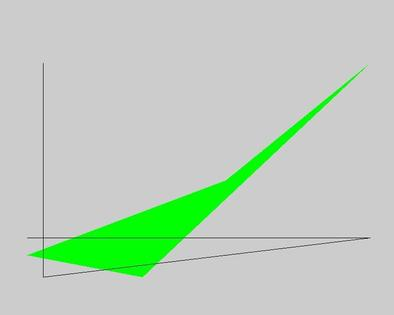
\includegraphics[scale=0.35]{2}
\end{center}


\begin{center}
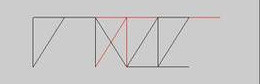
\includegraphics{1}
\end{center}

\section{Conclusões}
\label{sec:conclusao}

O grande objetivo do trabalho era o de produzir um jogo, o qual era composto por todo o código desenvolvido e ambiente gráfico (o qual não conseguimos desenvolver). Houveram duas tarefas nas quais não obtivemos pontuação máxima, e uma qual não conseguimos realizar (tarefa F). \par
Posto isto, consideramos que o grande objetivo não foi alcançado. Porém, conseguimos desenvolver grande parte de todo o código necessário para o funcionamento do jogo, restando apenas a implementação e adaptação deste numa interface gráfica funcional. \par
Consideramos também que todo este trabalho e desenvolvimento nos deu alguma aptidão para futuros desafios, desenvolvendo a nossa capacidade na interpretação de diferentes problemas. Organizou e estruturou a nossa forma de pensar, sendo cada vez mais "objetivos" e racionais no desenvolvimento de código. Foi, portanto, uma grande mais valia.

\end{document}